\chapter[Appendix]{Appendix}

\section*{Systemic Redshifts for HzRGs}

\begin{appendix}
The systematic velocities of the host galaxies in Chapter \ref{chapter4} are estimated from the \ion{He}{ii} $\lambda1640$ line. The line spectra are extracted from apertures of radius, $R=0.8$\arcsec where the \ion{He}{ii} line emission is sufficiently bright. A best-fit Gaussian solution is found for each line and the systematic redshift or velocity is inferred from the central wavelength of this fit. The figures in this section depict all the \ion{He}{ii} line fits for the seven high-redshift radio galaxies (HzRGs) in the sample. 

\begin{table*}
  \centering
  \caption[{HzRG sample redshifts and co-ordinates}]{Column (1) is the catalogue name of the HzRG, column (2) is the redshift estimated and column (3) are the co-ordinates the galaxy.}
  \label{table:hzrg-sample-chp4}
  \begin{tabular}{ l D{,}{\,\,\pm\,\,}{-3} l }
  & & \mc{} \\
   \hline \hline
  Galaxy & 
  \mc{Redshift} & 
  Co-ordinates ($\alpha, \delta$) \\
  & & (hms, dms) \\
  & & \mc{} \\
 \hline
MRC0943-242 		& 2.9228,0.0001	& 09:45:32.809, -24:28:49.848	 \\ 
  & & \mc{} \\
TN J0205+2422 		& 3.5050,0.0004 		& 02:05:10.690, 22:42:50.400	 \\ 
  & & \mc{} \\
TN J0121+1320		& 3.5181,0.0003 	 	& 01:21:42.730, 13:20:58.000	  \\
  & & \mc{} \\
4C+03.24 			& 3.5650,0.0006		& 12:45:38.360, 3:23:20.663   \\
  & & \mc{} \\
4C19.71				& 3.5892,0.0003 		& 21:44:06.976, 19:29:31.712	 \\	
  & & \mc{} \\	
TN J1338-1942		& 4.1077,0.0024		& 13:38:26.100, -19:42:31.100	  \\ 	
  & & \mc{} \\		
4C+04.11 			& 4.5082,0.0003 		& 03:11:48.004, 5:08:02.536	 \\ 
  & & \mc{} \\
 \hline
  \end{tabular}
\end{table*}

\begin{figure*}
\centering 
  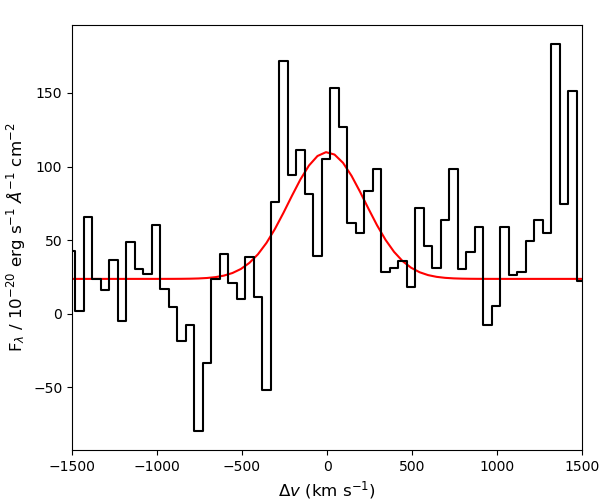
\includegraphics[width=0.5\textwidth]{plots_chp4/4C03_HeII.png}
  \caption[4C+03.24 \ion{He}{ii} line and best-fit]{{\bf 4C+03.24} \ion{He}{ii} $\lambda1640$ line and best-fit.}
\end{figure*}

\begin{figure*}
\centering
 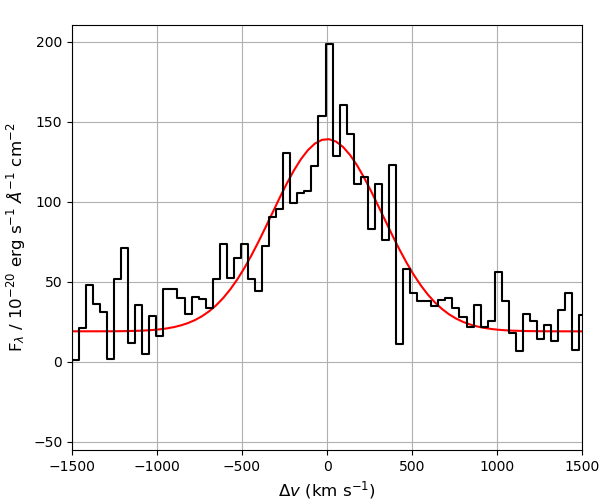
\includegraphics[width=0.5\textwidth]{plots_chp4/4C04_HeII.png}
 \caption[4C+04.11 \ion{He}{ii} line and best-fit]{{\bf 4C+04.11} \ion{He}{ii} $\lambda1640$ line and best-fit.}
\end{figure*}

\begin{figure*}
\centering
 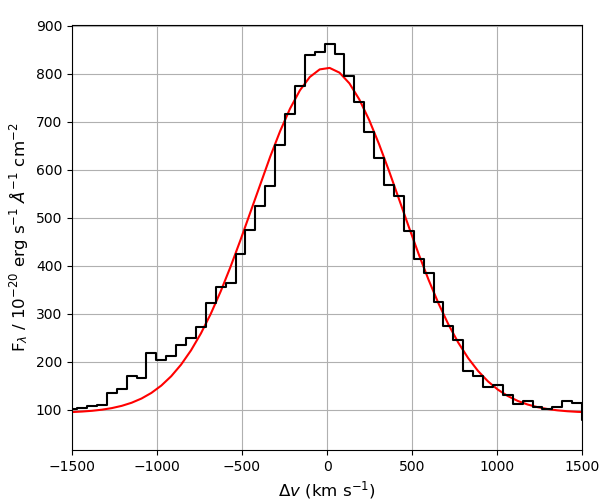
\includegraphics[width=0.5\textwidth]{plots_chp4/MRC0943_HeII.png}
 \caption[MRC 0943-242 \ion{He}{ii} line and best-fit]{{\bf MRC 0943-242} \ion{He}{ii} $\lambda1640$ line and best-fit.}
\end{figure*}

\begin{figure*}
\centering
   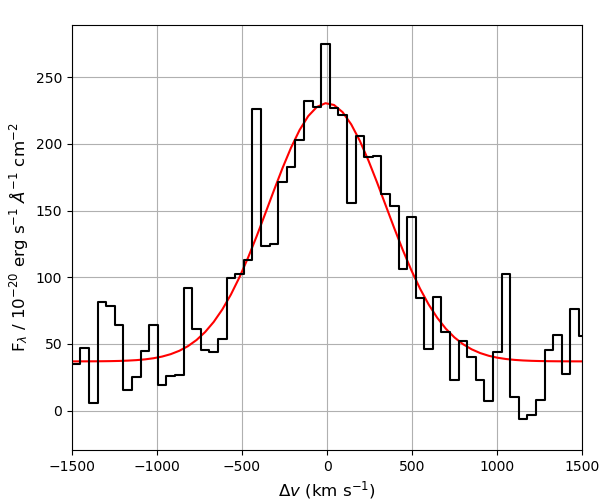
\includegraphics[width=0.5\textwidth]{plots_chp4/TN_J0121_HeII.png}
   \caption[TN J0121+1320 \ion{He}{ii} line and best-fit]{{\bf TN J0121+1320} \ion{He}{ii} $\lambda1640$ line and best-fit.}
\end{figure*}

\begin{figure*}
\centering
   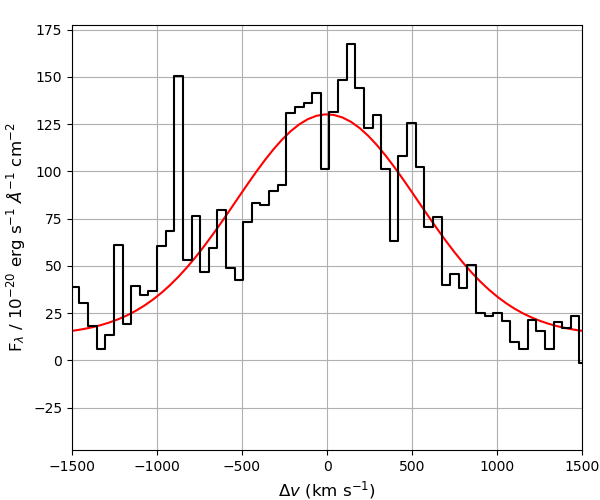
\includegraphics[width=0.5\textwidth]{plots_chp4/TN_J0205_HeII.png}
   \caption[TN J0205+2422 \ion{He}{ii} line and best-fit]{{\bf TN J0205+2422} \ion{He}{ii} $\lambda1640$ line and best-fit.}
\end{figure*}  

\begin{figure*}
\centering
 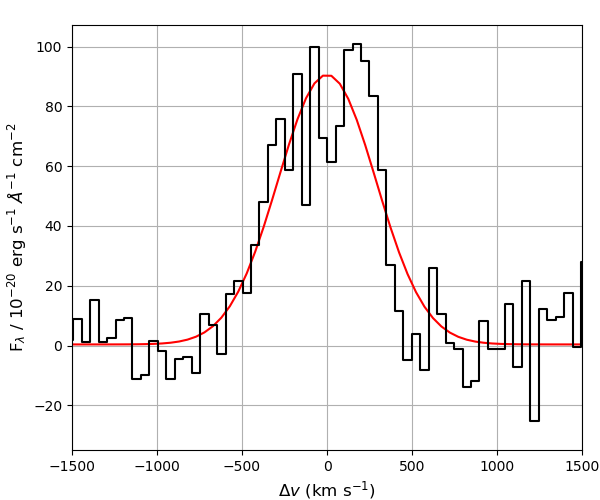
\includegraphics[width=0.5\textwidth]{plots_chp4/4C19_HeII.png}
 \caption[4C19.71 \ion{He}{ii} line and best-fit]{{\bf 4C19.71} \ion{He}{ii} $\lambda1640$ line and best-fit.}
\end{figure*}

\begin{figure*}
\centering
 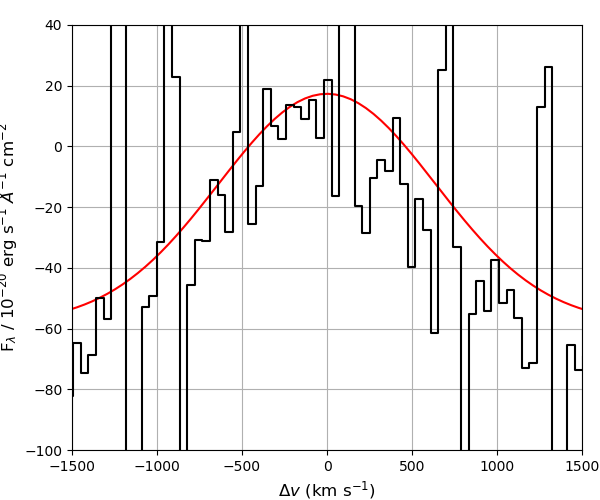
\includegraphics[width=0.5\textwidth]{plots_chp4/TNJ1338_HeII.png}
 \caption[TN J1338-1942 \ion{He}{ii} line and best-fit]{{\bf TN J1338-1942} \ion{He}{ii} $\lambda1640$ line and best-fit.}
\end{figure*}

\end{appendix}
